\label{chap:impl}
W~ostatnim rozdziale szczegółowo przedstawiony została implementacja aplikacji. Opisano użyte technologie i~metodologię, a~szczególną uwagę poświęcono problemom, które powstały podczas procesu tworzenia programu. Pierwsza sekcja zawiera opis środowiska, w~którym osadzona jest aplikacja, natomiast kolejne dwie skupiają się na dwóch logicznie wyodrębionych częściach projektu: uproszczonym formularzu edycyjnym oraz automatyzacji tworzenia haseł. W~ostatniej części rozdziału przedstawiono przebieg wdrożenia aplikacji w~polskim Wikisłowniku i~możliwości dalszego rozwoju.

Niniejszy rozdział zawiera odniesienia do plików źródłowych składających się na aplikację oraz pomocniczych. Wszystkie te pliki znajdują się na dołączonej do pracy płycie~CD w~katalogu \kod|src|.

\section{Wprowadzenie}
Oprogramowanie MediaWiki zostało napisane w~języku PHP (\emph{PHP Hypertext Preprocessor}) i~jest wysoce konfigurowalne za pomocą tzw. rozszerzeń, dodających kolejne funkcje --- przykładowo: obsługę przypisów, dodatkowe strony specjalne czy nowe funkcje parsera~\cite{mw:extensions}. W~projektach Fundacji obsługa rozszerzeń jest kontrolowana przez Fundację. Poszczególne projekty mogą składać prośby o~włączenie określonego rozszerzenia, decyzję podejmują zaś główni programiści Fundacji. Teoretycznie można rozważać utworzenie aplikacji dla Wikisłownika jako rozszerzenia w~PHP. Opcja ta została jednak odrzucona we wstępnej fazie projektu --- stworzenie rozszerzenia wymagałoby nieporównanie więcej formalności niż aplikacja kliencka, przede wszystkim jednak jego funkcjonalność byłaby znacznie ograniczona: poza polskim Wikisłownikiem żaden inny projekt nie mógłby z~niego skorzystać, na pewno nie zostałby więc włączony do głównej wersji MediaWiki.

\subsection{JavaScript w~Wikisłowniku}
Podobnie jak w~wielu innych przypadkach w~obrębie projektów Wikimedia jako metodę dostosowania silnika MediaWiki do szczególnych potrzeb wybrano zatem aplikację napisaną w~języku JavaScript. Konieczne jest zatem przedstawienie sposobu obsługi skryptów na stronach tych witryn. Pliki JavaScript ładowane są z~wielu różnych źródeł --- hierarchia w~nieco uproszczonej postaci jest następująca~\cite{de:js}:
\begin{enumerate}
	\item skrypty systemowe oprogramowania MediaWiki, wspólne dla wszystkich projektów oraz charakterystyczne dla danego projektu ze względu na ładowane rozszerzenia,
	\item skrypt zapisany na poziomie danego projektu jako strona \kod|MediaWiki:Common.js| --- dostęp do niego mają lokalni administratorzy,
	\item skrypt zapisany na poziomie danego projektu dla wybranej przez użytkownika skórki (domyślną jest \emph{Vector}, poprzednią był \emph{Monobook}) jako strona, np. \kod|MediaWiki:Vector.js| --- dostęp do niego mają lokalni administratorzy,
	\item tzw. gadżety, czyli dodatkowe skrypty rozszerzające funkcjonalność, możliwe do włączenia w~preferencjach użytkownika --- także one edytowane i~wybierane są przez administratorów,
	\item skrypt zapisany na stronie danego użytkownika, np. \kod|User:Sokrates/common.js| --- na tym poziomie możliwe jest dostosowywanie skryptów do swoich potrzeb przez każdego użytkownika,
	\item skrypt zapisany na stronie danego użytkownika dla wybranej skórki, np. dla skórki \emph{Vector} --- \kod|User:Sokrates/vector.js|.
\end{enumerate}
Jak widać, możliwości dołączania dodatkowych skryptów są elastyczne i~dostępne na różnych poziomach dla różnych użytkowników. Decyzja o~włączeniu skryptów dla wszystkich użytkowników danego projektu należy do jego administratorów (nie licząc wspólnych skryptów narzuconych przez Fundację), natomiast każdy użytkownik poprzez edycję specjalnej strony może uruchamiać różne skrypty na swoje potrzeby, nie będąc zmuszonym do korzystania z~dodatków do przeglądarek, takich jak Greasemonkey. W~ten sposób ułatwiony jest proces powstawania i~testowania nowych skryptów: osoby chcące przetestować nowy skrypt mogą na swojej stronie JS dołączyć go do swojej. Jeśli administratorzy uznają skrypt za wartościowy, mogą go dodać do zbioru gadżetów (wtedy każdy użytkownik ma możliwość włączenia skryptu bez konieczności edycji plików JS) lub do ogólnego pliku \kod|MediaWiki:Common.js|.

\subsubsection{MediaWiki 1.17}
Projekty Fundacji od czerwca 2011~roku używają wersji MediaWiki~1.17. Wersja ta wprowadziła kilka istotnych zmian, spośród których najważniejszą było wprowadzenie modułu \kod|ResourceLoader|, zmieniającego system ładowania dodatkowych plików, przede wszystkim skryptów i~arkuszy stylów~\cite{mw:117}. Wszystkie potrzebne pliki są łączone w~jeden i~dodatkowo kompresowane, dodatkowo poprawiono też obsługę pamięci podręcznej po stronie klienta. Do tej pory poszczególne pliki JS i~CSS przesyłane były statycznie w~wielu żądaniach HTTP, co mogło powodować problemy z~ich synchronizacją, a~przede wszystkim zwiększało obciążenie sieci. Aktualizacja software'u projektów Fundacji spowodowała konieczność aktualizacji większości używanych w~nich skryptów i~zaangażowała większość aktywnych uczestników zaznajomionych z~technikaliami~\cite{mw:migration}.

Od wersji~1.16 do MediaWiki dołączana jest biblioteka programistyczna jQuery, a~w~najnowszym wydaniu zaktualizowano ją do wersji 1.4.2~\cite{mw:jquery}. Jest to jedna z~najczęściej używanych bibliotek dla JavaScript, w~bardzo dużym stopniu usprawniająca programowanie w~tym języku. Kod pisany za jej pomocą jest o~wiele czytelniejszy i~prostszy, biblioteka pozwala też wyeliminować wiele problemów związanych z~nieprawidłową obsługą JavaScript w~niektórych przeglądarkach~\cite{jquery:action}~\cite{jquery:doc}.

\subsection{Środowisko programistyczne}
Programowanie w~JavaScript wymaga użycia innych metod niż tworzenie aplikacji desktopowych. Do tworzenia edytora dla Wikisłownika użyto m.in. następujących aplikacji:

\subsubsection{Geany}
Lekkie zintegrowane środowisko programistyczne (IDE)~\cite{geany}. W~początkowej fazie projektu używane było środowisko Eclipse z~dodatkowymi wtyczkami --- okazało się jednak, że obsługa JavaScript nie jest w~nim na tyle wygodna, aby konieczne było wykorzystywanie tak rozbudowanego edytora.
\subsubsection{Przeglądarki internetowe}
Aplikacja została przetestowana w~przeglądarkach Firefox $\geq$~4, Chrome 13, Opera $\geq$~10 i~Internet Explorer $\geq$~7, pod systemami operacyjnymi Linux i~Windows. Wyeliminowano błędy, które zostały odkryte w~czasie testów. W~trakcie implementacji używane były przeglądarki Google Chrome (i~jej wbudowane narzędzia deweloperskie) oraz Firefox z~dodatkiem Firebug, ułatwiającym debugowanie aplikacji~\cite{firebug}. Prawidłowe działanie aplikacji pod maksymalną możliwą liczbą dostępnych przeglądarek jest kluczowe ze względu na jej charakter --- edycja jest dostępna dla każdego użytkownika. Nie testowano jednak edytora w~starszych wersjach tych programów ze względu na ich znikome rozpowszechnienie i~niewspółmierny koszt takich testów w~stosunku do spodziewanych korzyści.
\subsubsection{Git}
Systemem kontroli wersji używanym w~projekcie był Git. Dzięki niemu możliwe było uniknięcie jakichkolwiek problemów związanych z~zarządzaniem wersjami. Dla bezpieczeństwa kod był na bieżąco wysyłany do zdalnego repozytorium założonym w~serwisie GitHub~\cite{github}. Kontroli wersji podlegała również niniejsza praca i~jej kod źródłowy w~systemie \XeTeX. Historia zmian aplikacji i~pracy jest dostępna do wglądu na serwerach GitHub~\cite{github:wikt}.
\subsubsection{The Regex Coach}
W~aplikacji duże znaczenie odgrywają wyrażenia regularne, wykorzystywane podczas parsowania wikitekstu. The Regex Coach jest programem ułatwiającym konstruowanie poprawnych wyrażeń~\cite{regexcoach}.
\spacer

\subsection{Dobre praktyki}
Nowy edytor został napisany za pomocą biblioteki jQuery, co ułatwia utrzymanie dobrej struktury. Kod podzielono na moduły funkcjonalne, co częściowo stanowi odpowiednik klasycznego paradygmatu obiektowego, często stosowany w~przypadku JavaScript. Język ten umożliwia pisanie aplikacji przy zachowaniu wielu różnych paradygmatów. W~przypadku opisywanej aplikacji zdecydowano się na wspomniany podział na moduły, będący pewnym kompromisem między paradygmatem funkcyjnym i~obiektowym. Moduły zaimplementowane są jako obiekty, których elementami są funkcje odpowiedzialne za operacje działające w~podobnym zakresie. Przykładowo parser wikitekstu jest modułem o~następującej strukturze:

\begin{jscode}{code:module}{Ogólna struktura modułu JavaScript}
var EParser = {
	getSections : function (code) {
		...
	},
	getSectionFromTitle : function (str) {
		...
	},
	getTitleFromCode : function (code) {
		...
	},
	...
};
\end{jscode}
Podział na moduły ułatwia uwzględnienie niektórych spośród licznych praktyk zalecanych przy programowaniu w~JavaScript. Istnieje kilka narzędzi, które w~automatyczny sposób badają jakość kodu w~tym języku, pomagając znaleźć potencjalne błędy i~uniknąć kolejnych. Podczas implementacji stale korzystano z~trzech z~nich: JSHint~\cite{jshint:doc}, JavaScriptLint~\cite{javascriptlint:doc}, a~przede wszystkim JSLint~\cite{jslint:doc}. Narzędzia te nie są do końca kompatybilne ze sobą nawzajem, dlatego za cel obrano całkowity brak ostrzeżeń generowanych przez JSLint. W~ten sposób udało się utrzymać m.in. następujące elementy:
\begin{itemize}
	\item kontrola nad zmiennymi globalnymi (w~przeciwieństwie do innych języków, np. PHP, domyślna deklaracja zmiennej bez słowa kluczowego \kod|var| powoduje umieszczenie jej w~zakresie globalnym),
	\item kończenie poleceń średnikiem (ich brak może prowadzić do błędów bardzo trudnych do wykrycia),
	\item odpowiednie tworzenie bloków kodu,
	\item sprawdzanie \kod|if (object.hasOwnProperty(name))| wewnątrz pętli \kod|for name in object| (z~powodu rozszerzalności prototypów funkcji brak takiego obostrzenia prowadzi do błędów),
	\item prawidłowe używanie operatorów takich jak \kod|===|, \kod|!==|,
	\item prawidłowe używanie konstruktorów,
	\item spójne wcięcia i~używanie nawiasów.
\end{itemize}

Istotnym zagadnieniem jest podział kodu na pliki. Podczas gdy w~trakcie implementacji oczywiste jest, że podział na moduły powinien implikować także podział na pliki, na cele testowania aplikacji przez społeczność o~wiele wygodniejsze jest używanie jednego pliku zawierającego jej całość --- w~przeciwnym razie konieczne byłoby stałe edytowanie większej liczby stron specjalnych Wikisłownika. Używanie wielu plików powoduje też problemy z~synchronizacją ich ładowania, ponieważ funkcja inicjalizująca aplikację powinna zostać uruchomiona dopiero po wczytaniu całości aplikacji.

Po rozważeniu kilku możliwości zdecydowano się na użycie skryptu \kod|make.sh| napisanego w~Bashu, łączącego wszystkie pliki aplikacji w~jeden, który okresowo był aktualizowany na stronie \url{http://pl.wiktionary.org/wiki/Wikipedysta:ToSter/ed.onefile.js}. Dodatkowym problemem było dołączenie kodu CSS: standardową metodą używaną w~Wikisłowniku byłoby utworzenie oddzielnej strony zakończonej na \kod|.css| i~ładowanie jej razem ze stroną \kod|.js|. W~skrypcie budującym wynikowy kod użyto jednak innej techniki --- arkusz stylów z~lokalnego pliku \kod|.css| był przetwarzany w~sposób umożliwiający dynamiczne dodanie go do zawartości strony jako łańcuch znaków. Skrypt \kod|make.sh| wykonywał też kilka innych czynności: opatrywał program adnotacjami dla JSLint, usuwał zbędne spacje i~znaczniki BOM w~plikach Unicode oraz zamykał całość aplikacji w~domknięciu JavaScript (\emph{closure}).

Kod aplikacji jest w~maksymalnie możliwym zakresie zgodny z~konwencjami przyjętymi przez programistów MediaWiki na potrzeby wewnętrznych części systemu~\cite{mw:conventions}.

\section{Formularz edycyjny}
\label{sec:impl-form}

Jedną z~dwóch głównych części aplikacji jest nowy formularz, usprawniający w~znacznym zakresie proces edycji i~tworzenia nowych artykułów. Do tej pory cały ów proces polegał na wpisywaniu, kopiowaniu i~uzupełnianiu wikikodu (por.~ilustracja~\ref{fig:plhaslo-edit}), a~najprostszym rozwiązaniem często okazywało się kopiowanie go z~innego, podobnego hasła i~modyfikowanie jedynie zmieniających się elementów. Dlatego też większość haseł w~Wikisłowniku powstawała seriami --- tworzenie pojedynczych haseł było niepraktyczne, natomiast wstawianie podobnego kodu do dziesiątek haseł dość łatwe do przeprowadzenia. Jako że każda sekcja językowa hasła składa się w~rzeczywistości z~par klucz--wartość, wygodniejszym sposobem wprowadzania danych byłby klasyczny formularz, do wypełniania jakiego przyzwyczajony jest każdy internauta. Nowy edytor został zatem zaprojektowany właśnie w~taki sposób, dzięki czemu zmniejsza się bariera wejścia dla początkującego redaktora. Od tej pory edycja hasła będzie polegać nie na wpisywaniu dość skomplikowanego kodu, co jest porównywalne z~prostym programowaniem, ale na wypełnieniu formularza.

Implementacja formularza składa się z~kilku modułów, spośród których główną rolę odgrywają \kod|EUi| w~pliku \kod|ed.ui.js| (interfejs użytkownika), \kod|EParser| i~\kod|ESectionParser| w~pliku \kod|ed.parser.js| (parser wikitekstu) oraz \kod|EPrinter| w~pliku \kod|ed.printer.js| (drukowanie danych przetworzonych przez aplikację). Poniżej opisano te moduły, szczególnie uwzględniając powstałe problemy i~ich rozwiązania.

\subsection{Interfejs użytkownika}
Kluczowym elementem projektu i~implementacji aplikacji jest interfejs użytkownika --- to jego jakość stanowi o~końcowym powodzeniu przedsięwzięcia. Szczególnie ważna jest bezproblemowa integracja nowego formularza z~dotychczasowym interfejsem. Wszystkie dotychczasowe funkcje używane w~trybie edycji, których zastosowanie miałoby sens i~w~nowej wersji, muszą pozostać dostępne.

Zrzuty ekranu nowego formularza załączono w~dodatku~\ref{app:screen}.

\begin{illustration}
	\fbox{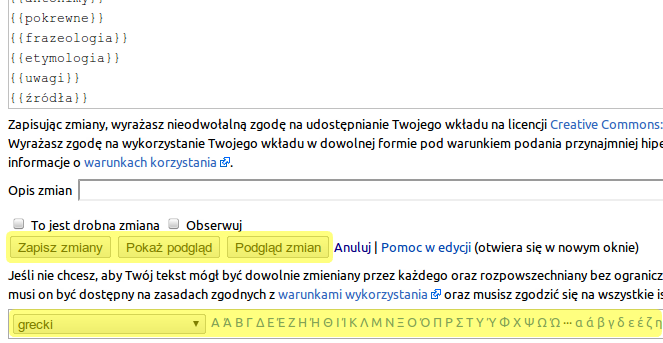
\includegraphics{edit-bottom-desc}}
	\caption{Kluczowe elementy interfejsu w~trybie edycji}
	\label{fig:edit-bottom}
\end{illustration}

Podstawowym problemem, powstałym na początku implementacji, było podpięcie nowego formularza pod mechanizmy przetwarzające dane po stronie serwera. Z~powodu braku jakiegokolwiek dostępu do konfiguracji serwera konieczne jest zapewnienie prawidłowego jego działania jedynie przy użyciu JavaScript. Na ilustracji~\ref{fig:edit-bottom} wyróżniono m.in. najważniejsze elementy sterujące edycją hasła. Są to trzy przyciski, których wybór powoduje wysłanie formularza w~trybie \kod|POST| na serwer do strony \kod|index.php| --- dalsze akcje uzależnione są od tego, który przycisk wybrano. Nową treścią hasła staje się zawartość głównego pola typu \kod|<textarea>|, o~identyfikatorze \kod|name="wpTextbox1"|. W~celu zapewnienia działania nowego formularza zgodnie z~oprogramowaniem MediaWiki możliwe były dwie opcje:
\begin{enumerate}
\item Usunięcie standardowych elementów, przede wszystkim pola \kod|wpTextbox1|, i~zastąpienie ich własnymi. Konieczne byłoby stworzenie pola formularza o~nazwie \kod|wpTextbox1| --- mogłoby to być pole ukryte (\kod|<input type="hidden" />|), które musiałoby być synchronizowane z~polami nowego formularza.
\item Ukrycie standardowych elementów i~synchronizacja zawartości pola \kod|wpTextbox1| z~polami nowego formularza.
\end{enumerate}
Wybór padł na rozwiązanie drugie z~kilku powodów. Okazało się, że dostęp do standardowych elementów w~trakcie działania nowego formularza jest bardzo przydatny, przede wszystkim zaś ich ukrywanie (za pomocą metody jQuery \kod|.hide()|, zmieniającej atrybut CSS \kod|display| na \kod|none|) umożliwia proste przełączanie między starym a~nowym formularzem w~trakcie edycji, co było jednym z~wymagań funkcjonalnych aplikacji. Należało zatem zapewnić prawidłową synchronizację pomiędzy polem \kod|wpTextbox1| a~polami nowego formularza. Najważniejsze było podpięcie odpowiednich zdarzeń pod przyciski wysyłające formularz na serwer, co widoczne jest na listingu~\ref{code:rebind}.

\begin{jscode}{code:rebind}{Funkcja \kod|EUi.rebindFormActions|}
rebindFormActions : function () {
    this.form.find('textarea').removeAttr('name');
    $('form').submit(function () {
	    if (EUi.usingNew) {
			EUi.deleteEmptySections();
			EUi.tbox.val(EPrinter.recalculateCode());
		}
		return true;
	});
}
\end{jscode}%$

W~momencie próby wysłania formularza na serwer skrypt sprawdza, czy użyty jest nowy formularz. W~takim przypadku ukryte okno tekstowe starego formularza, zapisane jako zmienna \kod|EUi.tbox|, wypełniane jest nową zawartością. Za jej obliczenie odpowiada funkcja \kod|EPrinter.recalculateCode|, opisana w~podsekcji~\ref{impl:parser}. Dzięki usunięciu atrybutów \kod|name| ze wszystkich pól tekstowych w~obrębie nowego formularza redukowana jest ilość przesyłanych danych, a~z~punktu widzenia serwera nic się nie zmienia.

Z~kolei po zmianach wprowadzonych za pomocą starego formularza konieczne jest ponowne parsowanie wikikodu, które jest wykonywane w~identyczny sposób jak przy inicjowaniu nowego edytora.

\begin{illustration}
	\fbox{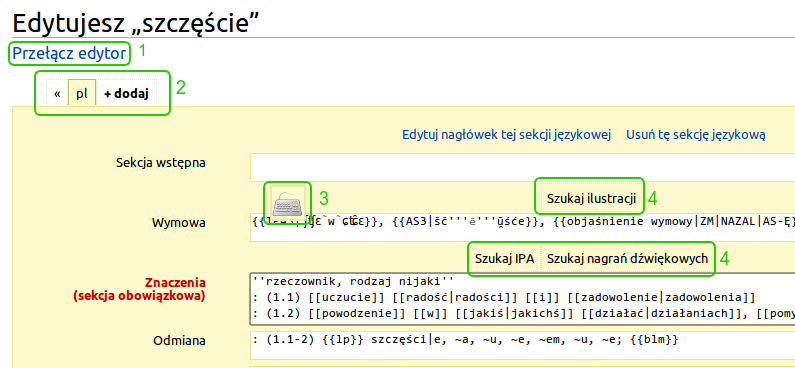
\includegraphics{newform-desc}}
	\caption{Fragment nowego formularza w~haśle z~jedną sekcją językową}
	\label{fig:newform}
\end{illustration}

Zrzut ekranu~\ref{fig:newform} przedstawia podstawowe elementy interfejsu nowego formularza:
\begin{enumerate}
\item Link pozwalający na przełączanie pomiędzy nowym a~starym edytorem,
\item Zakładki odpowiadające poszczególnym sekcjom językowym. Za podział na sekcje odpowiada moduł \kod|EParser|, natomiast zadaniem modułu \kod|EUi| jest ich odpowiednie wyświetlenie. Każdej sekcji odpowiada element \kod|<fieldset>| zawierający pola tekstowe z~poszczególnymi podsekcjami. Górne zakładki pozwalają na przełączanie pomiędzy sekcjami --- w~ten sposób redaktor widzi tylko tę sekcję, którą chce w~danym momencie edytować. W~starym formularzu konieczne było odnalezienie odpowiedniego kawałka kodu.

Sekcje językowe oznaczone są kodami ISO stosowanymi powszechnie w~Wikisłowniku. Oczywiście nie wszystkie kody są intuicyjne, dlatego po najechaniu myszą na każdą zakładkę pojawia się dokładna podpowiedź na temat danej sekcji.

Do zakładek językowych dodane są także zakładki o~specjalnej funkcji: pierwsza z~nich pozwala na edycję sekcji wstępnej (zawierającej m.in. interwiki), druga umożliwia dodanie nowej sekcji (pojawia się wówczas okno dialogowe z~zapytaniem o~język nowej sekcji).
\item Podręczna klawiaturka umożliwiająca wprowadzanie dużą liczbę znaków specjalnych do obecnie edytowanego pola. Podobna klawiaturka znajduje się w~starym edytorze --- została oznaczona kolorem żółtym na ilustracji~\ref{fig:edit-bottom}. W~nowym formularzu funkcja ta została usprawniona. Udało się wykorzystać istniejące już skrypty i~zintegrować z~aplikacją. Listing~\ref{code:specialchars} przedstawia moduł \kod|ESpecialChars|, odpowiadający za przemieszczanie elementów HTML pomiędzy nowym a~starym formularzem.
\item Przyciski pod poszczególnymi polami formularza pozwalają na automatyzację pewnych akcji. Ich działanie opisano w~sekcji~\ref{sec:impl-auto}.
\end{enumerate}

\begin{jscode}{code:specialchars}{Moduł \kod|ESpecialChars|}
ESpecialChars = {
	/* element HTML zawierajacy klawiaturke */
	obj : undefined,
	/* dotychczasowy element-rodzic klawiaturki */
	formerParent : undefined,
	detached : 0,

	/* odlaczenie klawiaturki od starego edytora i dodanie do elementu keyboard_keys w nowym formularzu */
	detach : function () {
		var container;
		if (ESpecialChars.detached) {
			return;
		}
		container = $('#keyboard_keys');
		ESpecialChars.obj = $('#editpage-specialchars');
		ESpecialChars.formerParent = ESpecialChars.obj.parent();
		ESpecialChars.obj.detach();

		container.append(ESpecialChars.obj);
		ESpecialChars.detached = 1;
	},

	/* ponowne przylaczenie klawiaturki do starego rodzica */
	attach : function () {
		if (!ESpecialChars.detached) {
			return;
		}
		EKeyboard.hide();
		ESpecialChars.obj.detach();
		ESpecialChars.formerParent.append(ESpecialChars.obj);
		ESpecialChars.detached = 0;
	},

	toggle : function () {
		if (ESpecialChars.detached) {
			ESpecialChars.attach();
		} else {
			ESpecialChars.detach();
		}
	}
};
\end{jscode}

Na ilustracji~\ref{fig:keyboard} pokazano działanie klawiaturki ekranowej w~nowym formularzu. Klawiaturę włącza się i~wyłącza kliknięciem w~ikonę z~klawiaturą, widoczną pod aktywnym właśnie polem tekstowym. Oprócz zawartości dostępnej w~starym formularzu można też wybrać jeden z~najczęściej używanych znaków. Ta funkcja znacząco usprawniła proces tworzenia haseł w~językach używających innych alfabetów lub znaków diakrytycznych. Stan klawiatury ekranowej (włączona/wyłączona) zapamiętywany jest w~ciasteczku przeglądarki, zostaje więce zachowany na kolejnych stronach.

\begin{illustration}
	\fbox{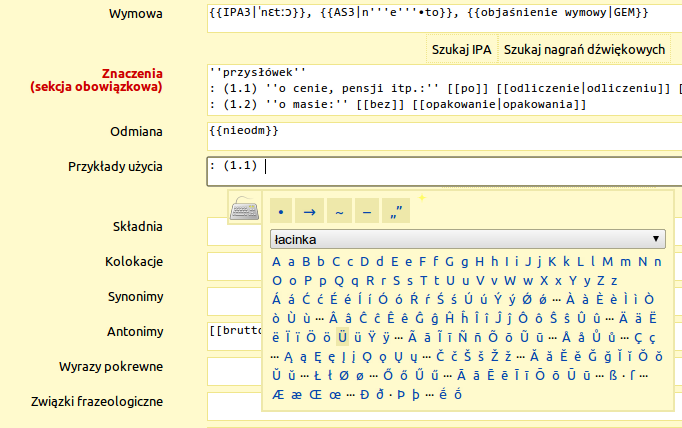
\includegraphics{edit-keyboard}}
	\caption{Użycie klawiaturki ekranowej w~nowym formularzu}
	\label{fig:keyboard}
\end{illustration}

Ciekawym problemem było ułożenie pól formularza w~taki sposób, by zajmował możliwie mało miejsca, a przy tym pozostał przejrzysty. Każda sekcja językowa składa się z~kilkunastu podsekcji, dlatego należało dobrze rozmieścić kilkanaście pól tekstowych, przy czym te mogły zawierać bardzo dużo tekstu (np. podsekcja \emph{tłumaczenia} w~popularnych polskich hasłach) albo i~pozostawać puste. Najprostszym, standardowym rozwiązaniem byłoby ustawienie stałej wysokości (np. równej 3~wierszom) dla każdego pola, które byłoby wyposażone w~zwykły pasek przewijania. Takie pola w~większości przypadków zajmowałyby jednak o~wiele za dużo miejsca, przy tym formularz z~dużymi białymi plamami jest niezbyt estetyczny. Zdecydowano się na rozwiązanie spotykane czasem w~portalach internetowych, najlepiej znane z~Facebooka --- pola tekstowe zmieniają swój rozmiar w~trakcie wpisywania kolejnych znaków. Istnieje kilka wtyczek do jQuery o~podobnej funkcjonalności, jednak na potrzeby aplikacji konieczne było stworzenie takiej, która łączy cechy kilku z~nich. Problemem okazała się też wydajność, ponieważ niektóre hasła mają w~trybie edycji nawet ponad sto pól dynamicznie dostosowujących swój rozmiar. Rozwiązaniem jest dołączenie do strony ukrytego elementu \kod|<div>|, do którego na bieżąco kopiowana jest zawartość ukrytego pola tekstowego --- na podstawie jego wysokości ustawiana jest wysokość pola. Kod przedstawiony jest na listingu~\ref{code:autoresize}.

\begin{jscode}{code:autoresize}{Wtyczka jQuery odpowiadająca za zmianę rozmiaru pól tekstowych}
/* wzorowane na https://github.com/jaz303/jquery-grab-bag/raw/master/javascripts/jquery.autogrow-textarea.js */
(function ($) {
	$.fn.autoresize = function () {
		var shadow = $('<div/>').css({
				position: 'absolute',
				top: -10000,
				left: -10000,
				resize: 'none'
			}).appendTo(document.body);

		this.filter('textarea').each(function () {
			var $this = $(this), minHeight = 25, maxHeight = 500,
				prevHeight = 0, nowHeight = 0;
			var update = function () {
				var val = this.value.replace(/[<>&]/g, 'w').replace(/\n$/, '<br/>&nbsp;').replace(/\n/g, '<br/>');
				shadow.html(val);
				nowHeight = Math.min(Math.max(shadow.height(), minHeight), maxHeight);
				if (nowHeight !== prevHeight) {
					$(this).css('height', nowHeight);
					EKeyboard.updatePosition($(this));
					prevHeight = nowHeight;
				}
			};

			shadow.css({
				width: $(this).width() - parseInt($this.css('paddingLeft'), 10) - parseInt($this.css('paddingRight'), 10),
				fontSize: $this.css('fontSize'),
				fontFamily: $this.css('fontFamily'),
				lineHeight: $this.css('lineHeight')
			});
			$(this).keyup(update).blur(update).focus(update);
			update.apply(this);
		});
		return this;
	};
}(jQuery));
\end{jscode}%$

Innymi usprawnieniami interfejsu użytkownika w~aplikacji są np.:
\begin{itemize}
\item Podpowiedzi pojawiające się po najechaniu myszką na część elementów strony. Aby ułatwić ich tworzenie, powstała wtyczka do jQuery. Dzięki jej użyciu aby dodać podpowiedź do dowolnego elementu HTML, wystarczyło nadać jej klasę CSS \kod|tip| i~treść podpowiedzi nadać za pomocą metody jQuery \kod|.data('tip', 'Odpowiedni tekst')|.
\item Okna dialogowe zastępujące standardowe funkcje typu \kod|alert|, \kod|confirm|, \kod|prompt|. Pojawiające się w~obrębie strony okno można dowolnie modyfikować.
\end{itemize}

\subsection{Parsowanie i~drukowanie wikitekstu}
\label{impl:parser}
Fundamentalne znaczenie dla aplikacji ma moduł odpowiadający za parsowanie wikitekstu --- kodu źródłowego haseł. O~trudności zagadnienia niech świadczy fakt, że przez ponad 10~lat istnienia Wikipedii nie udało się stworzyć edytora WYSIWYG --- i~prawdopodobnie w~dalszym ciągu nie będzie to wykonalne ze względu na coraz większy poziom skomplikowania artykułów. Tylko dzięki wyjątkowo przejrzystej strukturze polskiego Wikisłownika udało się stworzyć aplikację. Warto zaznaczyć, że kilka lat temu także polska edycja internetowego słownika nie nadawała się do tego typu projektu --- hasła udało się uprzątnąć za pomocą botów sterowanych przez kilka osób, które włożyły w~to dużo wysiłku.

Najistotniejszą funkcją parsera jest podział hasła na sekcje językowe, a~następnie na podsekcje --- zgodnie z~ogólnym schematem danego języka. Dzięki dobrej obsłudze wyrażeń regularnych w~JavaScript kod odpowiadający za to jest dość krótki, jednak stworzenie prawidłowo działającej aplikacji wymagało długich testów, przeprowadzanych zarówno przez autora, jak i~społeczność Wikisłownika.

O~ile parsowanie hasła odbywa się według jasnych reguł, o~tyle generowanie wikitekstu z~poszczególnych fragmentów artykułu okazało się o~wiele trudniejsze. Problemem nie było stworzenie kodu, który byłby poprawny, ale zadbanie o~to, by aplikacja nie powodowała zbędnych zmian w~kodzie. Kluczowa jest funkcja \kod|EPrinter.recalculateCode|, zaprezentowana w~wersji uproszczonej na listingu~\ref{code:recalculate}.

\begin{jscode}{code:recalculate}{Funkcja \kod|EPrinter.recalculateCode|}
recalculateCode : function () {
	var id, sec, i, j, subs,
		code = [],
		sortableSections = [];
	...
	/* sortableSections zawiera spis tych sekcji, ktore maja znalezc sie w hasle */
	/* kolejne kawalki kodu dodawane sa do tablicy code, ktora na koniec jest laczona w jeden lancuch znakow */
	for (i in sortableSections) {
		if (sortableSections.hasOwnProperty(i)) {
			sec = sortableSections[i];
			if (sec.id === EConstants.SECTION_ID_INTRO) {
				/* sekcja wstepna */
				/* EUi.val() pobiera zawartosc pola tekstowego w formularzu */
				code.push(EUi.val(EConstants.SECTION_ID_INTRO, '') + '\n');
			} else {
				/* tytul sekcji */
				code.push('== ' + sec.title + ' ==\n');
				/* poszczegolne podsekcje */
				for (j = 0; j < sec.subsections.length; j += 1) {
					subs = sec.subsections[j];
					if (subs.active) {
						subs.content = EUi.val(sec.id, subs.title);

						if (!subs.title && subs.content) {
							/* podsekcja wstepna */
							code.push(subs.content + '\n');
						} else if (subs.title && !subs.content) {
							/* pusta podsekcja */
							code.push('{{' + subs.title + '}}\n');
						} else ... {
							code.push('{{' + subs.title + '}}' + EPrinter.adequateWhitespace(subs) + subs.content + '\n');
						}
					}
				}
				code.push('\n');
			}
		}
	}
	/* laczenie w jeden napis i usuniecie wielokrotnych spacji */
	return $.trim(code.join('')).replace(/ {2,}/g, ' ');
}
\end{jscode}%$

Ciekawa jest funkcja \kod|EPrinter.adequateWhitespace|, użyta w~powyższym kodzie w~części odpowiadającej za wydrukowanie danej podsekcji. Jak się okazało, sposób drukowania poszczególnych podsekcji nie jest jednorodny. Za każdym razem istnieje kilka możliwości:
\begin{itemize}
\item Zawartość podsekcji zaczyna się od nowej linii.
\item Zawartość podsekcji zaczyna się od spacji.
\item Zawartość podsekcji zaczyna się od nowej linii i~dwukropka ze spacją (\kod|: |) powodującego wcięcie tekstu.
\end{itemize}

Aby ustalić, który wzorzec wybrać, trzeba wziąć pod uwagę wiele warunków. Na listingu~\ref{code:whitespace} przedstawiono funkcję to realizującą, opatrzoną dokładnymi komentarzami.

\begin{jscode}{code:whitespace}{Funkcja \kod|EPrinter.adequateWhitespace|}
adequateWhitespace : function (subsection) {
	var str = subsection.content;
	/*
	 * Teksty zaczynajace sie od dwukropka, gwiazdki, zaczynajace sie od "<references", "{{litera|", "{{kolor|", szablony zaczynajace sie na "{{zch-", linki do grafiki (file:, grafika: image: media: plik:, to samo duza litera, mozliwe biale znaki miedzy nawiasami kwadratowymi a tym slowem),...
	 */
	if (str.search(/[:\*#]|<references|\{\{(litera|kolor)\||\{\{zch-|\[\[(file|image|grafika|plik|media):/i) === 0) {
		return '\n';
	}
	/*
	 * ...teksty w polach "znaczenia", "przyklady" oraz "tlumaczenia" nie moga wystepowac zaraz po szablonie, jesli wystepuja, musza byc przeniesione bez dodawania dwukropka.
	 */
	if (EConstants.SUBSECTIONS_WITH_NL.indexOf(subsection.title) !== -1) {
		return '\n';
	}
	/*
	 * Inne teksty skladajace sie z wiecej niz jednej linii powinny byc przeniesione z dodaniem dwukropka i spacji na poczatku pierwszej linii
	 */
	if (str.indexOf('\n') !== -1 && str.search(/[:\*#]/) !== 0) {
		return '\n: ';
	}
	/*
	 * Wpp: dla wypelnionych przed edycja pol zachowujemy istniejace formatowanie, o ile dane pole juz bylo niepuste.
	*/
	if (subsection.initcontent) {
		return subsection.initmultiline ? '\n: ' : ' ';
	}
	/*
	 * w polach pustych przed edycja: w sekcjach "wymowa", "transliteracja", "transkrypcja", "ortografie", "klucz", "kreski", "czytania", "hanja-kreski" defaultem jest pisanie bezposrednio po szablonie (po spacji)...
	 */
	if (EConstants.SUBSECTIONS_WITHOUT_NL.indexOf(subsection.title) !== -1) {
		return ' ';
	}
	/*
	 * a w pozostalych od nastepnej linii (jesli nie jest to "znaczenie" ani pierwsza sekcja ani "przyklady", ani "tlumaczenia", a tekst nie zaczyna sie od dwukropka lub gwiazdki, to program powinien sam dodac dwukropek i spacje)
	 */
	return '\n: ';
}
\end{jscode}

Moduł \kod|EPrinter| odpowiada także za generowanie kodu z~danych pobranych w~sposób automatyczny. Niektóre z~tych funkcji zostały opisane w~kolejnej sekcji.

\section{Automatyzacja edycji hasła}
\label{sec:impl-auto}
Drugą funkcją obok uproszczenia ogólnego procesu edycji, jaką spełniać ma aplikacja, jest zautomatyzowanie niektórych działań wykonywanych przez redaktorów. W~sekcji~\ref{wikt:drawbacks} wspomniano o~dużym poziomie redundancji, będącym prostą konsekwencją rozbicia projektu na wersje językowe i~niemożności zachowania pierwszej postaci normalnej danych w~bazie Wikisłownika. Spora część danych wprowadzanych do haseł jest już obecna gdzie indziej --- czy to w~innych hasłach polskiego Wikisłownika, czy też w~innych wersjach językowych. Wielu redaktorów wykorzystuje przykładowo inne edycje projektu do wprowadzania danych takich jak wymowa w~międzynarodowym alfabecie fonetycznym (IPA), grafiki czy nagrania dźwiękowe, zaś na podstawie samej polskiej wersji możliwe jest chociażby kopiowanie przykładów użycia z~jednego hasła do drugiego.

\subsection{API MediaWiki}
Automatyzacja edytowania Wikisłownika (jak i~innych projektów Fundacji) byłaby niezwykle trudna bez interfejsu programistycznego dołączonego do każdej witryny opartej na MediaWiki~\cite{mw:api}. API umożliwia uproszczony dostęp do bazy Wikisłownika w~licznych formatach wymiany danych takich jak XML, JSON, YAML czy WDDX. Aby otrzymać odpowiedź na dowolne zapytanie, wystarczy pobrać dane z~adresu \url{http://pl.wiktionary.org/w/api.php} uzupełnionego o~odpowiednie parametry.

Ponieważ analogiczną funkcję ma każdy projekt Wikimedia, możliwe jest zautomatyzowane pobieranie informacji nawet z~kilkudziesięciu edycji językowych równocześnie. Przeszkodą w~przetwarzaniu tak pobieranych danych jest \emph{Same Origin Policy}, czyli koncepcja ograniczająca pobieranie danych za pomocą skryptów pomiędzy różnymi stronami internetowymi~\cite{mozilla:sop}. Z~tego powodu niemożliwe jest użycie większości formatów, w~tym XML. Sposobem na obejście niektórych ograniczeń jest użycie tzw. JSONP (lub JSON-P)~\cite{jsonp}. Jest to sposób na użycie istniejących technologii, który umożliwia pobieranie danych w~JavaScript z~innego serwera. Dane w~formacie JSON uzupełniane są na zdalnym serwerze o~wywołanie funkcji zdefiniowanej w~parametrze, z~którym skrypt został wywołany.

Istnieje kilka bibliotek, które mają ułatwiać operacje na API MediaWiki. Żadna z~nich jednak nie spełnia swojej roli w~odpowiedni sposób --- utrudnione jest dokonywanie kilku zapytań równocześnie, biblioteki bywają też przeładowane funkcjami, które nie są potrzebne w~projekcie dla Wikisłownika. Dlatego na jego potrzeby napisano od podstaw moduł \kod|EApi| (w~pliku \kod|ed.api.js|), będący integralną częścią aplikacji. Najistotniejsze funkcje modułu przedstawiono na listingu~\ref{code:api}.

\begin{jscode}{code:api}{Moduł \kod|EApi|}
EApi = {
	/* Zwraca adres URL dla danego jezyka i projektu */
	url : function (lang, project) {
		if (lang === undefined) {
			lang = 'pl';
		}
		if (project === undefined) {
			project = EConstants.WIKTIONARY;
		}
		return 'http://' + lang + '.' + project + '.org/w/api.php?';
	},

	/* Wykonanie zapytania pod danym adresem. Do podanych pol dolaczane sa standardowe */
	ask__prv : function (query, url) {
		if (url === undefined) {
			url = EApi.url();
		}
		query.action = 'query';
		query.format = 'json';
		query.meta = 'siteinfo';
		query.callback = 'EApi.callback';
		url += $.param(query);
		mw.loader.load(url);
	},

	/* Wykonanie pojedynczego zapytania */
	ask : function (query, callback, url) {
		if (EApi.waiting) {
			jAlert(EStr.WAITING_FOR_API);
			return -1;
		}
		EApi.waitingName = callback;
		EApi.waiting = 1;
		EApi.ask__prv(query, url);
		return 0;
	},

	/* Wykonanie kilku zapytan naraz */
	askMore : function (queries, callback) {
		var i, count = 0;

		if (EApi.waiting) {
			jAlert(EStr.WAITING_FOR_API);
			return -1;
		}
		EApi.waitingName = callback;

		for (i in queries) {
			if (queries.hasOwnProperty(i)) {
				count += 1;
			}
		}
		EApi.waiting = count;
		$.each(queries, function (url, query) {
			EApi.ask__prv(query, url);
		});
		return 0;
	},

	/* Funkcja wywolywana po nadejsciu pojedynczego rezultatu. Wynik zapytania dodawany jest do tablicy waitingResults. Jesli wszystkie rezultaty juz sie pojawily, wykonywana jest funkcja o nazwie zapisanej przedtem w zmiennej waitingName z argumentem waitingResults */
	callback : function (res) {
		var tmp = String(EApi.waitingName);
		EApi.waitingResults.push(res);
		EApi.waiting -= 1;
		if (!EApi.waiting) {
			EApi.waitingName = '';
			EUtil.executeFn(tmp, window, EApi.waitingResults);
			EApi.waitingResults = [];
		}
	},

	waiting : 0,
	waitingName : '',
	waitingResults : []
};
\end{jscode}

Najprostsze użycie modułu \kod|EApi| jest już nieskomplikowane: pozostaje zdefiniować dwie funkcje, z~których pierwsza odpowiada za przygotowanie i~wysłanie zapytania do wybranych projektów, druga zaś za przetworzenie i~wyświetlenie wyników. Wszystkie tego typu funkcje zebrano w~module \kod|EAutomator|. W~przyszłości możliwe jest podzielenie tego modułu na mniejsze, z~których każdy odpowiadałby konkretnemu zastosowaniu API MediaWiki. Funkcje przygotowane w~ramach opisywanej aplikacji opisano bardziej szczegółowo na kolejnych stronach.

\subsection{Funkcje automatyzujące edycję haseł}

\subsubsection{Aktualizacja interwiki}
Linki interwiki w~polskim Wikisłowniku aktualizowane są przez boty. Te działają sprawnie, jednak siłą rzeczy musi wystąpić opóźnienie między utworzeniem hasła a~dodaniem interwiki. Czasem redaktorowi przydatna byłaby wiedza o~innych wersjach językowych hasła, zanim linki do nich pojawią się w~artykule. Poniżej podano parametry zapytania, które zazwyczaj odnajdzie wszystkie wersje językowe.

\begin{opis}
\item[Projekty] Największe Wikisłowniki (angielski, hiszpański, francuski, niemiecki, rosyjski) oraz Wikisłowniki odpowiadające sekcjom językowym w~haśle
\item[Zapytanie]
\begin{verbatim}
query = {
	titles: mw.config.get('wgTitle'),
	prop: 'langlinks',
	lllimit: 200
};
\end{verbatim}
(Linki interwiki ze stron o~tytule równemu tytułowi obecnej strony)
\end{opis}

Poniżej przedstawiono kod odpowiadający za przetworzenie wyników i~aktualizację pola tekstowego zawierającego linki interwiki. Tak wygląda ogólny schemat funkcji wywoływanych po otrzymaniu rezultatów. W~przypadku innych funkcji zamiast podawania całego kodu omówione zostaną najciekawsze problemy.

\begin{jscode}{code:iw}{Funkcja \kod|EAutomator.fillInterwikiRe|}
fillInterwikiRe : function (results) {
	var iwikiString, curIwiki, re,
		iwikis = [];

	$.each(results, function () {
		var res = this;
		if (res.query === undefined || res.query.pages === undefined) {
			/* Nieprawidlowy wynik */
			return false;
		}
		$.each(res.query.pages, function (j, val) {
			if (j === '-1') {
				/* Indeks strony == -1 oznacza brak strony w danym projekcie */
				return false;
			}
			if (iwikis.indexOf(res.query.general.lang) === -1 && res.query.general.lang !== 'pl') {
				/* Do interwiki dodajemy dany projekt */
				iwikis.push(res.query.general.lang);
			}
			if (val.langlinks === undefined) {
				return false;
			}
			$.each(val.langlinks, function () {
				/* val.langlinks zawiera tytuly stron, do ktorych w danym projekcie wystepuja interwiki */
				if (this['*'] === mw.config.get('wgTitle') && iwikis.indexOf(this.lang) === -1 && this.lang !== 'pl') {
					iwikis.push(this.lang);
				}
			});
			return true;
		});
		return true;
	});
	/* sortowanie interwiki wedlug ustalonego klucza */
	iwikis.sort(function (a, b) { return EConstants.INTERWIKI_ORDER.indexOf(a) - EConstants.INTERWIKI_ORDER.indexOf(b); });
	/* przygotowanie lancucha znakow ze wszystkimi interwiki */
	iwikiString = $.map(iwikis, function (val) {
		return '[[' + val + ':' + mw.config.get('wgTitle') + ']]';
	}).join(' ');
	curIwiki = $('#ed_0000_').val();
	if (curIwiki === '') {
		/* dotad sekcja wstepna byla pusta */
		/* .autoresize() powoduje dostosowanie wysokosci pola */
		$('#ed_0000_').val(iwikiString).autoresize();
	} else {
		/* zastapienie poprzedniej wersji */
		re = new RegExp('(\\[\\[[a-z\\-]+' + ':' + mw.config.get('wgTitle') + '\\]\\]\\s*)+');
		$('#ed_0000_').val($.trim(iwikiString + curIwiki.replace(re, '\n'))).autoresize();
	}
	EApi.done(EConstants.MODE_IW);
}
\end{jscode}

\subsubsection{Pobieranie zapisu wymowy w~IPA}
Zapis wymowy w~międzynarodowym alfabecie fonetycznym (IPA) to jedna z~tych informacji, które można bez problemu przenosić pomiędzy różnymi wersjami językowymi Wikisłownika. Często zdarza się, że w~wielu wersjach językowych zapis pewnego słowa jest podany, brakuje go zaś w~polskiej edycji. Najczęściej IPA nie jest ręcznie wpisywane do hasła, ale kopiowane z~innego źródła --- jest to oczywiście wygodniejsze z~powodu konieczności używania innego alfabetu. Aby ułatwić wstawienie tej informacji do hasła, można poprzez API pobrać zawartość haseł z~interwiki. Ważne jest, by dobrze sparsować otrzymane hasła w~poszukiwaniu IPA.

\begin{opis}
\item[Projekty] Wikisłowniki odpowiadające sekcjom językowym w~haśle i~inne z~linków interwiki
\item[Zapytanie]
\begin{verbatim}
query = {
	titles: mw.config.get('wgTitle'),
	prop: 'revisions',
	rvprop: 'content'
};
\end{verbatim}
(Zawartość stron o~tytule równemu tytułowi obecnej strony)
\end{opis}

Hasła w~innych wersjach językowych mogą dotyczyć wielu języków, w~których występuje dane słowo. Koniecznie trzeba zminimalizować więc ryzyko wstawienia wymowy wyrazu w~innym języku niż w~obecnie edytowanej sekcji przez niedoświadczonego użytkownika. Przy okazji implementacji funkcji odpowiadającej za przetworzenie wyników okazało się, że programistyczny podział hasła na sekcje w~innej wersji językowej wcale nie musi być tak prosty jak w~wersji polskiej. Choć wspólne dla projektów jest stosowanie nagłówków dla poszczególnych języków, to w~części wersji nagłówki te są generowane dynamicznie przez szablony. Przykładowo nagłówek sekcji języka polskiego w~Wikisłowniku hiszpańskim ma postać \kod@{{PL-ES|Nazwa}}@, a~w~Wikisłowniku francuskim: \kod@== {{=pl=}} ==@.

Wydaje się, że dobrym rozwiązaniem problemu jest podanie przy każdej wykrytej informacji o~IPA w~obcojęzycznej wersji hasła także nagłówka sekcji, w~której ją znaleziono. Co prawda istnieją Wikisłowniki takie jak wietnamski, gdzie nie sposób wyodrębnić poszczególne sekcje, jednak dla większości udało się to osiągnąć. W~ten sposób redaktor otrzymuje zawartość nagłówka, która pozwala się zorientować, o~jaki język może chodzić.

Ponieważ w~większości wersji językowych zapisy IPA podawane są w~określonym szablonie, przy użyciu funkcji pomocniczych odnajdujących parametry szablonów udało się doprowadzić do pobierania IPA z~kilkunastu Wikisłowników. Listing pokazuje, jak różnorodne są sposoby podawania IPA.

\begin{jscode}{code:ipa}{Funkcja \kod|EAutomator.extractIPA|}
extractIPA : function (str, lang) {
	switch (lang) {
	case 'en': case 'cs': case 'sk': case 'it': case 'af': case 'ko': case 'nl':
	case 'co': case 'vi': case 'ga': case 'is': case 'li': case 'lv': case 'no':
	case 'sl': case 'ja': case 'simple':
		return EAutomator.extractFirstArgsFromTemplates(str, 'IPA', lang);
	case 'fr': case 'mg': case 'oc':
		return EAutomator.extractFirstArgsFromTemplates(str, 'pron', lang);
	case 'de':
		return EAutomator.extractFirstArgsFromTemplates(str, 'Lautschrift', lang);
	case 'es':
		return EAutomator.extractAllArgsFromTemplates(str, 'pronunciación', lang);
	case 'ca':
		return EAutomator.extractSecondArgsFromTemplates(str, 'pron', lang);
	case 'ro':
		return EAutomator.extractFirstArgsFromTemplates(str, 'AFI', lang);
	case 'et':
		return EAutomator.extractFirstArgsFromTemplates(str, 'hääldus', lang);
	case 'el':
		return EAutomator.extractFirstArgsFromTemplates(str, 'ΔΦΑ', lang);
	case 'eo':
		return EAutomator.extractFirstArgsFromTemplates(str, 'IFA', lang);
	case 'tl':
		return EAutomator.extractFirstArgsFromTemplates(str, 'API', lang);
	case 'ru':
		return EAutomator.extractIPA_ru(str);
	default:
		return [];
	}
}
\end{jscode}

Dodatkową komplikacją jest występowanie IPA w~dwóch wariantach. Zapis w~nawiasach kwadratowych to zapis fonetyczny, natomiast między ukośnikami --- zapis fonologiczny. W~różnych wersjach językowych używane są różne warianty, natomiast w~polskiej edycji podawane są oba. Aplikacja bierze pod uwagę, jak zbudowany jest szablon w~danym Wikisłowniku, i~w~zależności od tego pozwala na wstawienie IPA w~szablonie \kod|{{IPA}}| lub \kod|{{IPA3}}|.

Za wyświetlenie zapisów IPA, które można następnie wstawić jednym kliknięciem, odpowiedzialna jest funkcja \kod|EPrinter.ipaResult|. Jej efektem jest pojawienie się okienka, z~którego można wybrać odpowiedni zapis (patrz ilustracja~\ref{fig:iparesult}). Nagłówki sekcji językowych, z~których pochodzą IPA, wyświetlane są po najechaniu myszką.

\begin{illustration}
	\fbox{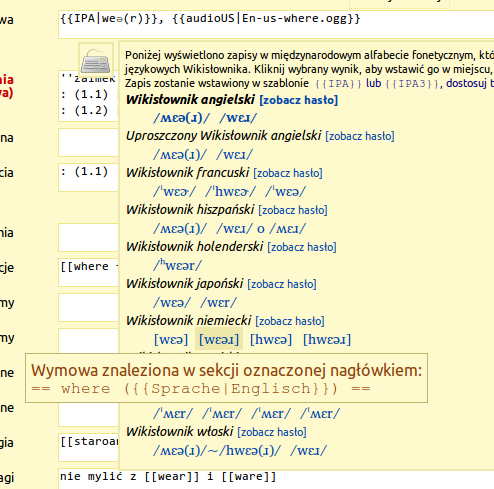
\includegraphics[width=0.7\textwidth]{iparesult}}
	\caption{Fragment okna wyświetlającego pobrane zapisy IPA}
	\label{fig:iparesult}
\end{illustration}

\subsubsection{Pobieranie grafik}

\subsubsection{Pobieranie nagrań wymowy}

\subsubsection{Pobieranie przykładów użycia}

\section{Wdrożenie i~dalszy rozwój}
\label{sec:impl-deploy}

...
%licencja
%IE < Win7 :(
